\documentclass[12pt]{amsart}
% packages
\usepackage{graphicx}
\usepackage{setspace}
\usepackage{amssymb,amsmath,amsthm,amsfonts,amscd}
\usepackage{hyperref}
\usepackage{color}
\usepackage{booktabs}
\usepackage{tabularx}
\usepackage{enumitem}
\usepackage[retainorgcmds]{IEEEtrantools}
\usepackage[notref,notcite,final]{showkeys}
\usepackage[final]{pdfpages}
\usepackage{fancyhdr}
\usepackage{upgreek}
\usepackage{multicol}
\usepackage{fontawesome}
\usepackage{halloweenmath}
% set margin as 0.75in
\usepackage[margin=0.75in]{geometry}

% tikz-related settings
\usepackage{tkz-berge}
\usetikzlibrary{calc,quotes}
\usetikzlibrary{arrows.meta}
\usetikzlibrary{positioning, automata}
\usetikzlibrary{decorations.pathreplacing}

%% For table
\usepackage{tikz}
\usetikzlibrary{tikzmark}

% theorem environments with italic font
\newtheorem{thm}{Theorem}[section]
\newtheorem*{thm*}{Theorem}
\newtheorem{lemma}[thm]{Lemma}
\newtheorem{prop}[thm]{Proposition}
\newtheorem{claim}[thm]{Claim}
\newtheorem{corollary}[thm]{Corollary}
\newtheorem{conjecture}[thm]{Conjecture}
\newtheorem{question}[thm]{Question}
\newtheorem{procedure}[thm]{Procedure}
\newtheorem{assumption}[thm]{Assumption}

% theorem environments with roman font (use lower-case version in body
% of text, e.g., \begin{example} rather than \begin{Example})
\newtheorem{Definition}[thm]{Definition}
\newenvironment{definition}
{\begin{Definition}\rm}{\end{Definition}}
\newtheorem{Example}[thm]{Example}
\newenvironment{example}
{\begin{Example}\rm}{\end{Example}}

\theoremstyle{definition}
\newtheorem{remark}[thm]{\textbf{Remark}}

% special sets
\newcommand{\A}{\mathbb{A}}
\newcommand{\C}{\mathbb{C}}
\newcommand{\F}{\mathbb{F}}
\newcommand{\N}{\mathbb{N}}
\newcommand{\Q}{\mathbb{Q}}
\newcommand{\R}{\mathbb{R}}
\newcommand{\Z}{\mathbb{Z}}
\newcommand{\cals}{\mathcal{S}}
\newcommand{\ZZ}{\mathbb{Z}_{\ge 0}}
\newcommand{\cala}{\mathcal{A}}
\newcommand{\calb}{\mathcal{B}}
\newcommand{\cald}{\mathcal{D}}
\newcommand{\calh}{\mathcal{H}}
\newcommand{\call}{\mathcal{L}}
\newcommand{\calr}{\mathcal{R}}
\newcommand{\la}{\mathbf{a}}
\newcommand{\lgl}{\mathfrak{gl}}
\newcommand{\lsl}{\mathfrak{sl}}
\newcommand{\lieg}{\mathfrak{g}}

% math operators
\DeclareMathOperator{\kernel}{\mathrm{ker}}
\DeclareMathOperator{\image}{\mathrm{im}}
\DeclareMathOperator{\rad}{\mathrm{rad}}
\DeclareMathOperator{\id}{\mathrm{id}}
\DeclareMathOperator{\hum}{[\mathrm{Hum}]}
\DeclareMathOperator{\eh}{[\mathrm{EH}]}
\DeclareMathOperator{\lcm}{\mathrm{lcm}}
\DeclareMathOperator{\Aut}{\mathrm{Aut}}
\DeclareMathOperator{\Inn}{\mathrm{Inn}}
\DeclareMathOperator{\Out}{\mathrm{Out}}
\DeclareMathOperator{\Gal}{\mathrm{Gal}}


% frequently used shorthands
\newcommand{\ra}{\rightarrow}
\newcommand{\se}{\subseteq}
\newcommand{\ip}[1]{\langle#1\rangle}
\newcommand{\dual}{^*}
\newcommand{\inverse}{^{-1}}
\newcommand{\norm}[2]{\|#1\|_{#2}}
\newcommand{\abs}[1]{\lvert #1 \rvert}
\newcommand{\Abs}[1]{\bigg| #1 \bigg|}
\newcommand\bm[1]{\begin{bmatrix}#1\end{bmatrix}}
\newcommand{\op}{\text{op}}

% nicer looking empty set
\let\oldemptyset\emptyset
\let\emptyset\varnothing

%the var phi gang
\let\oldphi\phi
\let\phi\varphi

\setlist[enumerate,1]{topsep=1em,leftmargin=1.8em, itemsep=0.5em, label=\textup{(}\arabic*\textup{)}}
\setlist[enumerate,2]{topsep=0.5em,leftmargin=3em, itemsep=0.3em}

%pagestyle
%\pagestyle{fancy} 

\begin{document}
\begin{center}
    \textsc{Math 501. HW 14\\ Ian Jorquera\\ Collaborators: The people I work with }
\end{center}
\vspace{1em}
% See http://www.mathematicalgemstones.com/maria/Math501Fall22.php
% for problems

% sage: https://sagecell.sagemath.org/
\begin{itemize}

\item[(1)] % (1)
One of my favorite bijections is Foata's bijection. However I also don't like this bijection as it is too simple but also caused me much trouble. My other favorite bijection is any and all sign reversing involutions. These are so cool.\\

\item[(2)] % (1)
we can see that Fraklin's Involution does in fact act as an involution for $(7,6,4,3)$\\
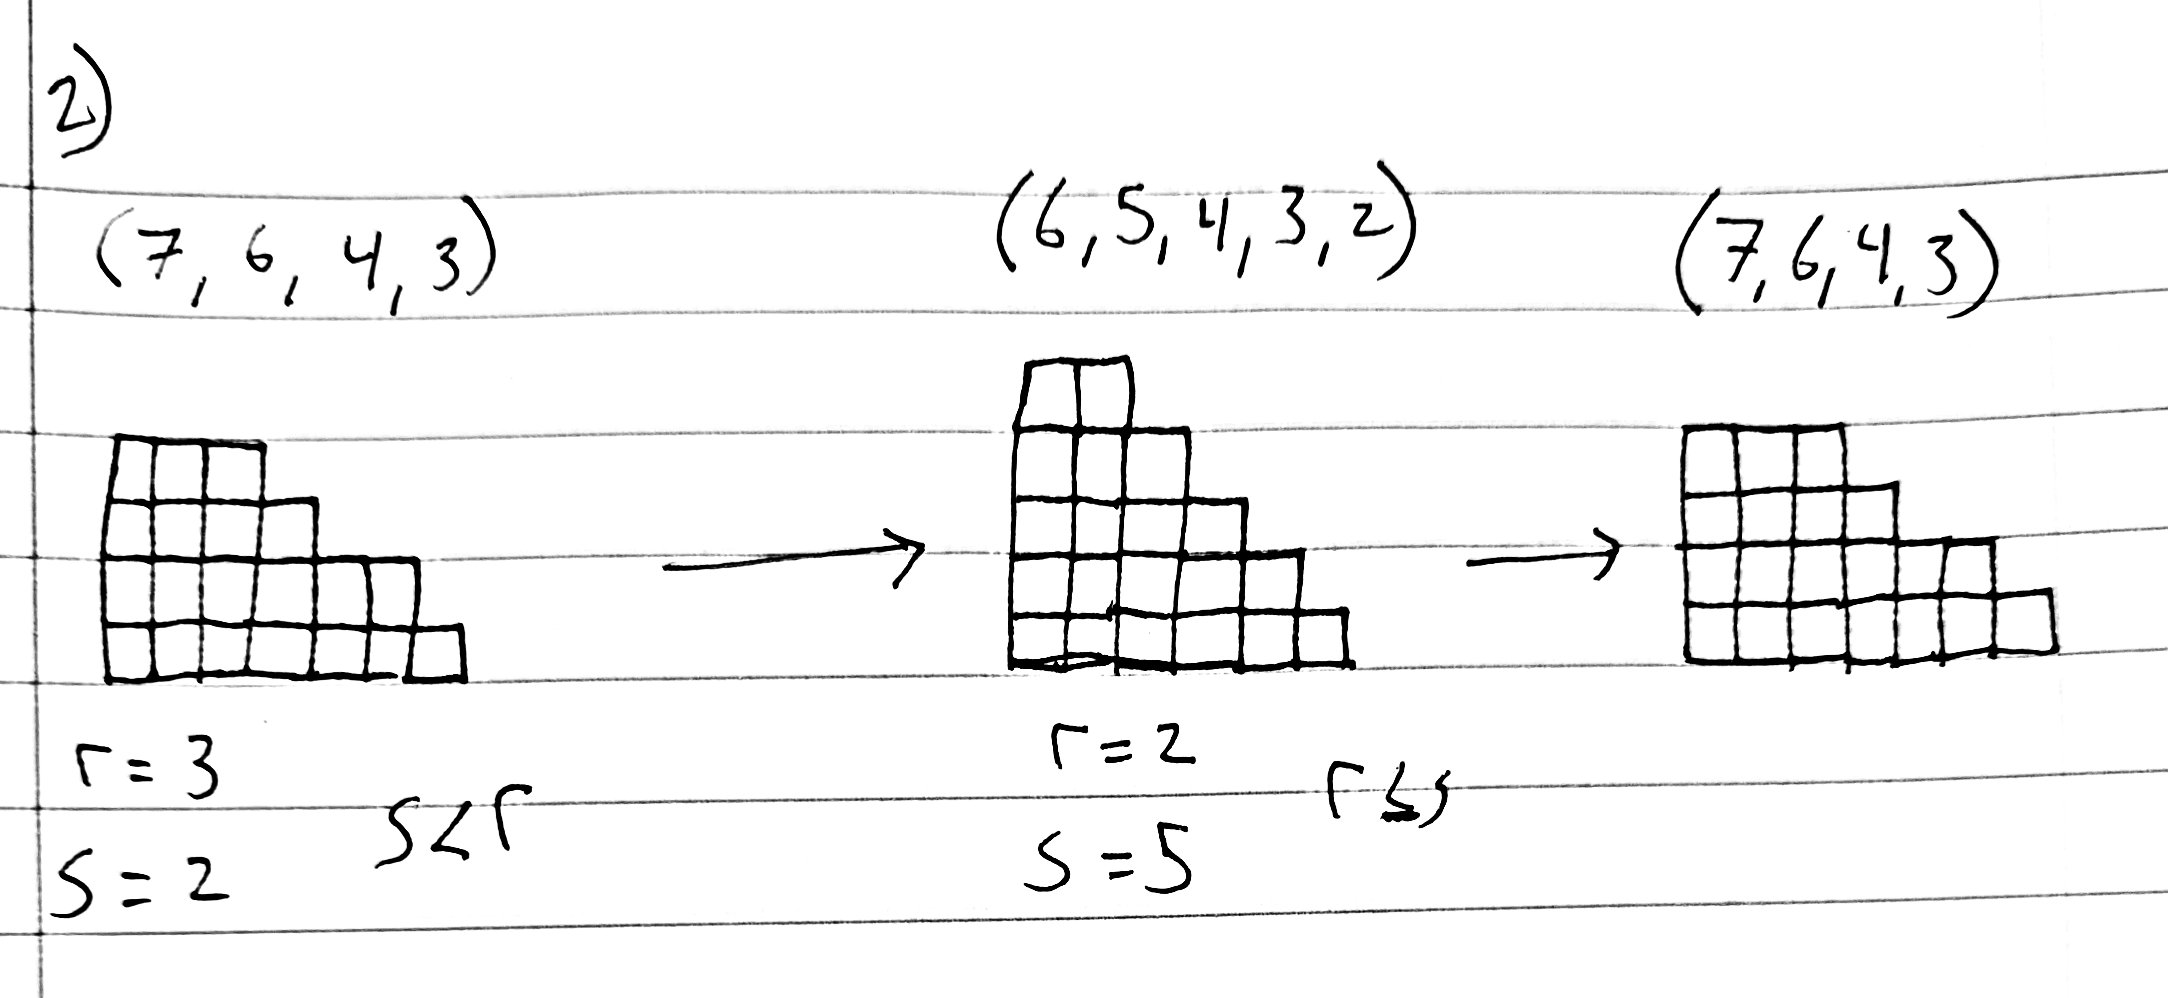
\includegraphics[width=.9\textwidth]{202212011629101000.jpg}

\item[(3)] % sagan 16c (2)
The number of partitions with largest part being size $k$ corresponds to the generating function that picks a part of size $k$, ie with $x^k$, then picking any number of blocks of size $1$, which corresponds to $(1+x^1+x^2+\dots)=\frac{1}{1-x}$. Then we can pick any number of parts with blocks of size $i$ where $1\leq i \leq k$ which is $(1+x^i+x^{2i}+\dots)=\frac{1}{1-x^i}$. This means the generating function would be the product of these and so $\frac{x^k}{(1-x)(1-x^2)\cdots (1-x^k)}$.\\

We can then show that the generating function for the number of partitions with $k$ parts is the same generating function. To see this consider the involution of conjugating of the Young Tableau. Which would map a partition with biggest part $k$ to a partition with $k$ parts notice that. Furthermore this is an inverse as conjugating would then take an involution with $k$ parts to a partition with biggest part $k$. So we know that the generating functions for the number of partitions of $k$ parts is in bijection with the number of partitions with biggest part $k$ and so their generating functions are the same. \\

\item[(4)] % saga 16d.  (3)
First we will create a generating function for the number of partitions of $n$ with biggest block being of size at most $k$. In this case it is the same as from problem $3$ excpet we will no longer require that we pick a block of size $k$, meaning the generating function is $\frac{1}{(1-x)(1-x^2)\cdots (1-x^k)}$. And because this is the same as adding up the generating function for partitions of $n$ with biggest part of size $i$, where $0\leq i\leq k$ which is the same as adding up the generating function for partitions of $n$ into $i$ parts, where $0\leq i\leq k$, we know that the number partitions of $n$ into at most $k$ blocks is the same generating function.\\

Here to create a generating function for partitions of size $n$ we can sum over all derfee squares of size $d\geq 0$, which will correspond to the term $x^{d^2}$ counting the number of blocks of the $d$ derfee square. For any derfee square we can also pick addition blocks to add to the right side of the derfee square. Because there are $d$ rows we need to add blocks that correspond to a partition with at most $d$ blocks whose generating function is $\frac{1}{(1-x)(1-x^2)\cdots (1-x^k)}$. we can also add blocks above the derfee square, each of which can be at most size $d$, and so we need to add blocks that correspond to a partition with biggest block at most $d$ which has the generating function, $\frac{1}{(1-x)(1-x^2)\cdots (1-x^d)}$ These terms together correspond to the generating function the the number of partitions of $n$ with a $d$ derfee square.\\

\item[(8)] % (3)
The generating function for the number of partitions with odd parts is the product of picking $1$s, then picking $3$, then picking $5$, and so on. This gives us the generating function being the product $$\sum_{i=1}^{\infty} p_o(n)x^n= (1+x+x^2+\dots)(1+x^3+x^6+\dots)(1+x^5+x^{10}+\dots)\dots=\prod_{i=1}^\infty \frac{1}{1-x^{2i-1}}$$
We want to show that the generating function 

$${\sum_{i=1}^{\infty} p_o(n)x^n=\prod_{i=1}^\infty \frac{1}{1-x^{2i-1}}}\text{ and }{\sum_{i=0}^\infty q(n)x^n=\prod_{i=1}^{\infty}(1+x^i)}$$
are the same. We will do this by showing they have the same reciprocal $\prod_{i=1}^{\infty}\frac{1}{1+x^i}$. From class we know that $\prod_{i=1}^{\infty}(1+x^i)\prod_{i=1}^{\infty}(1-x^{2k-1})=1$ and so $\prod_{i=1}^{\infty}\frac{1}{1+x^i}\prod_{i=1}^{\infty}\frac{1}{1-x^{2k-1}}=1$. Notice also that $\prod_{i=1}^{\infty}\frac{1}{1+x^i}\prod_{i=1}^{\infty}(1+x^i)=1$. And so we know that these generating functions are equal and so $p_o(n)=q(n)$.


\end{itemize}

\end{document}





















\documentclass[12pt]{amsart}
% packages
\usepackage{graphicx}
\usepackage{setspace}
\usepackage{amssymb,amsmath,amsthm,amsfonts,amscd}
\usepackage{hyperref}
\usepackage{color}
\usepackage{booktabs}
\usepackage{tabularx}
\usepackage{enumitem}
\usepackage[retainorgcmds]{IEEEtrantools}
\usepackage[notref,notcite,final]{showkeys}
\usepackage[final]{pdfpages}
\usepackage{fancyhdr}
\usepackage{upgreek}
\usepackage{multicol}
\usepackage{fontawesome}
\usepackage{halloweenmath}
% set margin as 0.75in
\usepackage[margin=0.75in]{geometry}

% tikz-related settings
\usepackage{tkz-berge}
\usetikzlibrary{calc,quotes}
\usetikzlibrary{arrows.meta}
\usetikzlibrary{positioning, automata}
\usetikzlibrary{decorations.pathreplacing}

%% For table
\usepackage{tikz}
\usetikzlibrary{tikzmark}

% theorem environments with italic font
\newtheorem{thm}{Theorem}[section]
\newtheorem*{thm*}{Theorem}
\newtheorem{lemma}[thm]{Lemma}
\newtheorem{prop}[thm]{Proposition}
\newtheorem{claim}[thm]{Claim}
\newtheorem{corollary}[thm]{Corollary}
\newtheorem{conjecture}[thm]{Conjecture}
\newtheorem{question}[thm]{Question}
\newtheorem{procedure}[thm]{Procedure}
\newtheorem{assumption}[thm]{Assumption}

% theorem environments with roman font (use lower-case version in body
% of text, e.g., \begin{example} rather than \begin{Example})
\newtheorem{Definition}[thm]{Definition}
\newenvironment{definition}
{\begin{Definition}\rm}{\end{Definition}}
\newtheorem{Example}[thm]{Example}
\newenvironment{example}
{\begin{Example}\rm}{\end{Example}}

\theoremstyle{definition}
\newtheorem{remark}[thm]{\textbf{Remark}}

% special sets
\newcommand{\A}{\mathbb{A}}
\newcommand{\C}{\mathbb{C}}
\newcommand{\F}{\mathbb{F}}
\newcommand{\N}{\mathbb{N}}
\newcommand{\Q}{\mathbb{Q}}
\newcommand{\R}{\mathbb{R}}
\newcommand{\Z}{\mathbb{Z}}
\newcommand{\cals}{\mathcal{S}}
\newcommand{\ZZ}{\mathbb{Z}_{\ge 0}}
\newcommand{\cala}{\mathcal{A}}
\newcommand{\calb}{\mathcal{B}}
\newcommand{\cald}{\mathcal{D}}
\newcommand{\calh}{\mathcal{H}}
\newcommand{\call}{\mathcal{L}}
\newcommand{\calr}{\mathcal{R}}
\newcommand{\la}{\mathbf{a}}
\newcommand{\lgl}{\mathfrak{gl}}
\newcommand{\lsl}{\mathfrak{sl}}
\newcommand{\lieg}{\mathfrak{g}}

% math operators
\DeclareMathOperator{\kernel}{\mathrm{ker}}
\DeclareMathOperator{\image}{\mathrm{im}}
\DeclareMathOperator{\rad}{\mathrm{rad}}
\DeclareMathOperator{\id}{\mathrm{id}}
\DeclareMathOperator{\hum}{[\mathrm{Hum}]}
\DeclareMathOperator{\eh}{[\mathrm{EH}]}
\DeclareMathOperator{\lcm}{\mathrm{lcm}}
\DeclareMathOperator{\Aut}{\mathrm{Aut}}
\DeclareMathOperator{\Inn}{\mathrm{Inn}}
\DeclareMathOperator{\Out}{\mathrm{Out}}
\DeclareMathOperator{\Gal}{\mathrm{Gal}}


% frequently used shorthands
\newcommand{\ra}{\rightarrow}
\newcommand{\se}{\subseteq}
\newcommand{\ip}[1]{\langle#1\rangle}
\newcommand{\dual}{^*}
\newcommand{\inverse}{^{-1}}
\newcommand{\norm}[2]{\|#1\|_{#2}}
\newcommand{\abs}[1]{\lvert #1 \rvert}
\newcommand{\Abs}[1]{\bigg| #1 \bigg|}
\newcommand\bm[1]{\begin{bmatrix}#1\end{bmatrix}}
\newcommand{\op}{\text{op}}

% nicer looking empty set
\let\oldemptyset\emptyset
\let\emptyset\varnothing

%the var phi gang
\let\oldphi\phi
\let\phi\varphi

\setlist[enumerate,1]{topsep=1em,leftmargin=1.8em, itemsep=0.5em, label=\textup{(}\arabic*\textup{)}}
\setlist[enumerate,2]{topsep=0.5em,leftmargin=3em, itemsep=0.3em}

%pagestyle
%\pagestyle{fancy} 

\begin{document}
\begin{center}
    \textsc{Math 501. HW 14\\ Ian Jorquera\\ Collaborators: The Usual: Kaylee, Kylie, Sarah, Ignacio and Ian }
\end{center}
\vspace{1em}
% See http://www.mathematicalgemstones.com/maria/Math501Fall22.php
% for problems

% sage: https://sagecell.sagemath.org/
\begin{itemize}

\item[(1)] % (1)
One of my favorite bijections is Foata's bijection. However I also don't like this bijection as it is too simple but also caused me much trouble. My other favorite bijection is any and all sign reversing involutions. These are so cool.\\

\item[(3)] % sagan 16c (2)
First we will create a generating function for the number of partitions of $n$ with biggest block being of size at most $k$. In this case it is the same as from problem $$

Here to create a generating function for partitions of size $n$ we can sum over all derfee squares of size $d\geq 0$, which will correspond to the term $x^{d^2}$ counting the number of blocks of the $d$ derfee square. For any derfee square we can also pick addition blocks to add to the right side of the derfee square. Because there are $d$ rows we need to add blocks that correspond to a partition with at most $d$ blocks whose generating function is $\frac{1}{(1-x)(1-x^2)\cdots (1-x^k)}$. we can also add blocks above the derfee square, each of which can be at most size $d$, and so we need to add blocks that correspond to a partition with biggest block at most $k$ which has the generating function, $\frac{1}{(1-x)(1-x^2)\cdots (1-x^k)}$ These terms together correspond to the generating function with a $d$ derfee square.

\item[(8)] % (3)
The generating function for the number of partitions with odd parts is the product of picking $1$s, then picking $3$, then picking $5$, and so on. This gives us the generating function being the product $$\sum_{i=1}^{\infty} p_o(n)x^n= (1+x+x^2+\dots)(1+x^3+x^6+\dots)(1+x^5+x^{10}+\dots)\dots=\prod_{i=1}^\infty \frac{1}{1-x^{2i-1}}$$
We want to show that the generating function 

$${\sum_{i=1}^{\infty} p_o(n)x^n=\prod_{i=1}^\infty \frac{1}{1-x^{2i-1}}}\text{ and }{\sum_{i=0}^\infty q(n)x^n=\prod_{i=1}^{\infty}(1+x^i)}$$
are the same. We will do this by showing they have the same reciprocal $\prod_{i=1}^{\infty}\frac{1}{1+x^i}$. From class we know that $\prod_{i=1}^{\infty}(1+x^i)\prod_{i=1}^{\infty}(1-x^{2k-1})=1$ and so $\prod_{i=1}^{\infty}\frac{1}{1+x^i}\prod_{i=1}^{\infty}\frac{1}{1-x^{2k-1}}=1$. Notice also that $\prod_{i=1}^{\infty}\frac{1}{1+x^i}\prod_{i=1}^{\infty}(1+x^i)=1$. And so we know that these generating functions are equal and so $p_o(n)=q(n)$.


\end{itemize}

\end{document}


